%% 
%% Copyright 2007, 2008, 2009 Elsevier Ltd
%% 
%% This file is part of the 'Elsarticle Bundle'.
%% ---------------------------------------------
%% 
%% It may be distributed under the conditions of the LaTeX Project Public
%% License, either version 1.2 of this license or (at your option) any
%% later version.  The latest version of this license is in
%%    http://www.latex-project.org/lppl.txt
%% and version 1.2 or later is part of all distributions of LaTeX
%% version 1999/12/01 or later.
%% 
%% The list of all files belonging to the 'Elsarticle Bundle' is
%% given in the file `manifest.txt'.
%% 

%% Template article for Elsevier's document class `elsarticle'
%% with numbered style bibliographic references
%% SP 2008/03/01

\documentclass[review,12pt]{elsarticle}

%% Use the option review to obtain double line spacing
%% \documentclass[authoryear,preprint,review,12pt]{elsarticle}

%% Use the options 1p,twocolumn; 3p; 3p,twocolumn; 5p; or 5p,twocolumn
%% for a journal layout:
%% \documentclass[final,1p,times]{elsarticle}
%% \documentclass[final,1p,times,twocolumn]{elsarticle}
%% \documentclass[final,3p,times]{elsarticle}
%% \documentclass[final,3p,times,twocolumn]{elsarticle}
%% \documentclass[final,5p,times]{elsarticle}
%% \documentclass[final,5p,times,twocolumn]{elsarticle}

%% For including figures, graphicx.sty has been loaded in
%% elsarticle.cls. If you prefer to use the old commands
%% please give \usepackage{epsfig}

%% The amssymb package provides various useful mathematical symbols
\usepackage{amssymb}
%% The amsthm package provides extended theorem environments
%% \usepackage{amsthm}
\usepackage{amsmath}
\usepackage{pdflscape} 
\usepackage{threeparttable}
\usepackage{longtable}
\usepackage{booktabs}

%% The lineno packages adds line numbers. Start line numbering with
%% \begin{linenumbers}, end it with \end{linenumbers}. Or switch it on
%% for the whole article with \linenumbers.
%% 
\usepackage{lineno}

\journal{JCOMM}

\begin{document}

\begin{frontmatter}

  \title{What Nearby and Deferred Quotes Tell Us about Linkages and Adjustments
to Information}

  
  \begin{abstract}
  The recent `Financialization' of commodity futures markets, increases in
  biofuel production, and climate change potentially have imposed profound
  shifts in the way commodity futures markets operate. This article
  examines the corn market quote-by-quote to develop metrics on liquidity
  and transmission of information. The metrics are based on insights
  derived from sequential trading models on single securities, index
  futures on a basket of securities, and special features of commodity
  futures markets. Correlation between quote revisions in nearby and
  deferred contracts measure information-based activity, and correlations
  between revisions of the time lagged nearby and deferred maturity
  measure the speed at which information is transmitted among the
  different futures maturities. Information-based trading results in near
  perfect correlation between revisions to bids and offers in nearby and
  deferred contracts. Within one second, information is fully transmitted
  from nearby to deferred contracts.
  \end{abstract}
   \begin{keyword} market, microstructure, information, electronic trading \sep \end{keyword}
 \end{frontmatter}

\begin{linenumbers}

\section{Introduction}\label{introduction}

There has been recent concern about whether and how the
`Financialization of Commodity Markets' has impacted market efficiency
and efficacy in the traditional roles of risk mitigation, coordinating
production, and coordinating consumption through time (S. H. Irwin and
Sanders 2011; Cheng and Xiong 2013; S. H. Irwin and Sanders 2012;
Henderson, Pearson, and Wang 2015). Further, the recent increase in the
production of biofuel from food commodities and volatile crude oil
prices has changed the relationship between food and energy commodities
(Serra and Zilberman 2013; M. L. Mallory, Irwin, and Hayes 2012;
Gardebroek and Hernandez 2013; Vacha et al. 2013; Avalos 2014;
Trujillo-Barrera et al. 2012). Additionally, climate change, rising
demand for agricultural commodities, and volatile inventories and
exchange rates have imposed structural changes in commodity markets
(Balcombe, Prakash, and others 2011; Gilbert and Morgan 2010; A.
Prakash, Gilbert, and others 2011).

These issues represent potentially profound shifts in the way commodity
markets operate, and the articles cited above have considered their
implications. However, how these changes affect commodity markets on a
tick-by-tick and quote-by-quote basis needs to be considered. Since
global price discovery occurs on global futures exchanges for the major
food commodities, a detailed consideration of these changes on trading
activity, patterns, and consequences is warranted. We use ``high
frequency data'' (time stamped to the second), in order to capture
faster price change adjustments taking place after significant technical
developments in trading platforms in the second half of the 2000s,
characterized by high speed trading.

Price analysis can be classified into structural and non-structural
studies. While structural models rely on economic theory, non-structural
analyses identify empirical regularities in the data. The approach
throughout this article is non-structural. We employ this approach
primarily because there is scant market microstructure literature
developed with the particular characteristics of commodity futures
markets in mind. In this article, we are motivated to develop initial
metrics of information-based activity in commodity markets. We
anticipate this work will lead to future developments in the
microstructure of commodity markets literature.

Even how to develop simple metrics of information-based activity from
standard microstructure models is not obvious because standard models of
trading securities are not necessarily directly applicable to commodity
futures markets. For example, in commodities futures markets several
contracts with different maturities trade in the marketplace, each
reacting to information- and liquidity-motivated trades. Each contract
responds to information-based shocks because there is a cost to store
the physical commodity through time (Working 1948; Working 1949; Brennan
1958). Further, each contract maturity attracts different levels of
liquidity, and it is not known what impact a lack of liquidity has on
information transmission up the forward curve.

The metrics we develop in this article on liquidity and transmission of
information are based on insights we combined from the sequential
trading models on single securities, index futures based on a basket of
securities, and some of the features of commodity futures markets
described in the preceding paragraph. Using the standard sequential
trading result that quote revisions only occur if liquidity providers
have updated their beliefs about the value of the security after
observing order flows, the correlation between quote revisions in nearby
and deferred contracts can be used to measure information-based
activity, and correlations between revisions of the time lagged nearby
and deferred maturity can be used to measure the speed at which
information is transmitted among the different futures maturities. This
metric is sensible in commodity futures markets but not in a market for
a single security, because futures markets have multiple maturity
contracts that should respond to information in a very similar and
predictable way.

Garcia and Leuthold (1992) examined how USDA announcements are
transmitted in nearby and deferred contracts. Using daily price
observations and USDA announcement dates, they observe that deferred
futures responses are similar to nearby harvest futures, but the
information effect is somewhat smaller. Information appears to affect
prices over a horizon of at least five days. Informatively, they call
for closer examination of intra-day data to develop a more comprehensive
understanding of price behavior. In contrast to the results found by
Garcia and Leuthold, we find information is fully transmitted within one
second, reflecting a market that is highly efficient in transmitting
information up the forward curve from nearby to distant contract
maturities.

The remainder of the article is organized as follows. First, we provide
a background of the sequential trading and index futures microstructure
literature and describe the conceptual framework that motivates our
interpretation of correlations of quote revisions as a metric of
information-based activity. Next we describe the data and report the
results of our analysis. Finally, we offer concluding remarks.

\section{Literature Review}\label{literature-review}

The literature on how information affects liquidity in securities
markets is long and rich.\footnote{The interested reader can refer to
  O'Hara (1995) for an excellent and detailed overview of the evolution
  of this literature.} Bagehot (1971) is regarded as the first to
demonstrate that a bid-ask spread (BAS) arises when asymmetric
information is present even if inventory and transactions costs are
assumed to be zero. Copeland and Galai (1983) build on Bagehot's work by
assuming that a specific proportion of traders are informed. Knowing
this, the market maker adjusts his quoted bids and offers to maximize
expected profit. Copeland and Galai's model, however, does not account
for the fact that the trades themselves can reveal information about
whether or not traders are informed. Glosten and Milgrom (1985)
formalize this concept and develop a model where the market maker
adjusts his beliefs based on the trades that occur. The market maker
knows that at least some of the traders are informed so sell orders
revise the market maker's belief downward about the value of the
security and buy orders revise his belief upward. They show that the
spread is increasing in the proportion of informed traders, and there is
a point at which too many informed traders require the market maker to
set the spread so wide, that trade does not occur and the market halts
(an example of the famous ``Market for Lemons'' described by Akerlof
(1970)).

Easley and O'Hara (1987) and Easley and O'Hara (1992) incorporate trade
size and its effect to a model similar to Glosten and Milgrom. A market
maker must set breakeven bid and offer quotes knowing that he faces a
certain proportion of informed traders who only trade if they receive a
signal that an information event has occurred, and a certain proportion
of uninformed traders who do not receive an information signal but
occasionally need to trade for liquidity reasons. Both informed and
uninformed traders can choose between a large and small block trading
size. This model setup leads to two types of equilibria: a separating
equilibrium where informed traders only trade in large quantities and a
pooling equilibria where informed traders may trade both large and small
quantities. This model setup of information uncertainty and asymmetric
information leads to the market maker updating his beliefs about the
value of the security (and therefore his quotes) based on the order flow
he observes in the market. For example, in a separating equilibrium a
large trading block causes the market maker to revise upward his
expectation that an information event has occurred (since informed
traders do not transact at small sizes). This contrasts with the pooling
equilibrium where informed traders place small orders to prevent the
market maker from updating his beliefs that an information event has
occurred.

Hasbrouck (2006) provides an overview of how Easley, Hvidkjaer, and
O'Hara (2002) and Easley, Kiefer, and O'Hara (1997) use the Easley and
O'Hara models of informed trading to develop a measure of the
probability of informed trading (PIN). This measure, though, is
estimated solely based on the sequence of order arrivals, where a trade
is labeled as buyer initiated if the trade occurs above the midpoint of
the quoted spread and seller initiated if the trade occurs below the
midpoint of the quoted spread. Numerous studies have documented that
there may be problems with downward bias in the estimated PIN (Yan and
Zhang 2012; Vega 2006; Boehmer, Grammig, and Theissen 2007) and
estimating information-based trading in this way ignores some aspects of
futures markets discussed above that are not present in securities
markets. For these reasons we seek an alternative to the PIN measure of
information-based trading in commodity futures.

To our knowledge, there are no market microstructure models that
explicitly take into account the features of commodity futures markets.
The closest models come from work on index futures that cover a basket
of securities. Most prominent is the work by Kumar and Seppi (1994) who
assume \emph{N} different non-dividend paying securities and an index
futures contract on a buy-and-hold portfolio of a subset of these
stocks. In Kumar and Seppi's model, specialists in the cash market
observe a signal, and floor traders of the futures index observe a
signal about the value of the index but not the individual securities. A
key feature they build into the model is a lag in the information
transmittal between the cash and futures markets because specialists
only observe order flows from their own market, and not the other. This
lag in information transmittal allows for arbitrageurs, who possess
faster telecommunication technologies, to learn from transactions in
both markets and make profitable trades in the cash and futures markets.
These arbitrageurs are analogous to spread traders who trade in both
nearby and deferred futures contracts hoping to profit on relative price
movements.

There are some important distinctions between the arbitrageurs as
proposed in the Kumar and Seppi model and spread traders in a futures
market. Namely, the basis between a composite of cash security prices
and the price of a futures index of the same basket should behave in
very predictable ways (the basis, in theory, should only vary with
interest rates and expected changes in dividend yields if information is
symmetric). In contrast, the spread between the prices of two commodity
futures contracts with different maturities depends on many more
uncertain structural variables: e.g., domestic and international
consumption, exchange rates, production or distribution bottlenecks, or
weather. The arbitrageurs in Kumar and Seppi's model need only to wait
for others in the marketplace to learn to profit. The futures market
spread trader entertains much more risk in betting on relative price
changes between two futures maturities.

In the next section we draw insights from the sequential trading models
described above to generate empirical predictions about the correlations
between revisions to bids and offers of nearby and deferred maturity
commodity futures contracts.

\section{Conceptual Framework}\label{conceptual-framework}

In this section we develop a conceptual framework for how the role of
liquidity-based activity versus information-based activity should affect
quote revisions in a commodity futures market. Using insights from the
Easley and O'Hara models, along with features of commodity futures
markets, we generate empirical predictions about the correlations
between revisions to quotes in the nearby and deferred maturity
commodity futures contracts.

First, consider an absence of information. In the Easley and O'Hara
sequential trader models, the market maker revises his quotes only when
he updates his belief that the value of the security has changed.
Therefore, we interpret no changes in revisions to bids (offers) as
indicative of no information having arrived to the market. Any
transactions that occur at these prices, the market maker believes are
conducted by uninformed traders demanding liquidity.

Conversely, when we observe revisions to the bid or offer, we can infer
that the market maker from the Easley and O'Hara models has updated
beliefs about information arrival to the market based on past order
flows. These revisions to the bid and offer we interpret as indicative
of information arriving to the market.

Now we discuss features of futures markets that we can utilize when
considering revisions to nearby and deferred contract quotes. First, in
actively traded commodity futures markets there is no market maker, but
there are entities who actively supply liquidity to the market under a
variety of motives. Since the Easley and O'Hara models consider a
competitive market maker, it is irrelevant whether there is one market
maker in the traditional sense or a large number of traders providing
liquidity. Second, when market makers revise their beliefs that an
information event has arrived to the market, they know it affects
futures contracts of all maturities so quotes must be revised in all
contracts.

This should induce a high degree of correlation between bid and offer
revisions when an information event arrives. Further, one market maker
would revise bids and offers on futures contracts of all maturities at
the same time they update beliefs about an information event having
occurred. As a practical matter, many independent traders provide
liquidity to the market at any given time, so it is not clear that the
Bayesian updating described in the Easley and O'Hara models will happen
in all maturities simultaneously. Therefore, it is of interest to
consider the relationship between revisions to quotes in the nearby
contract at different time lags) and revisions to quotes in deferred
maturity contracts.

\section{Data}\label{data}

The data used in this analysis come from the CME Group's Top of Book
(BBO) database for Globex corn futures quotes and transactions from
01/14/2008-11/4/2011. The data contain the best bid, bid size, best
offer, offer size, last trade price, and last trade size of the order
book for each active futures contract, time-stamped to the second.

Table 1 shows the first ten entries to our data after manipulating the
raw BBO data set from CME Group to display the entire top of the book on
one line with the appropriate time stamp. The first column is the
time-stamp, the second column is the trade sequence number, which the
CME Group gives to individual trades to identify separate orders that
arrive on the same second. The third column, SYMBOL, identifies which
futures maturity the observation represents. In this case, 1003 stands
for March 2010, with the first two characters representing the year and
the second two characters representing the month. The fourth column,
OFRSIZ, is the number of contracts quoted at the best offer price. The
fifth column, OFR, is the best offered price. The sixth column, BIDSIZ,
is the number of contracts quoted at the best bid price; the last
column, BID, is the best bid price. For each date in our sample, we
consider the first to mature (nearby), one, two, and three contracts
deferred. We define the nearby contract to be the next contract to
expire unless the date was after the 20th of the month prior to
expiration. Then we roll the nearby to the next to expire contract. We
rolled the series on the 20th to avoid decreasing volume as the contract
neared the delivery period. We also excluded the September futures
contract from our analysis because of low trading volume.\footnote{September
  experiences low trading volumes because deliveries on this contract
  sometimes (but not usually) can come from early new crop harvest,
  making its price relative to the traditional new crop contract,
  December, hard to predict.}

Figure 1 displays average transaction price per day, number of revisions
to the ask, number of revisions to the bid, and number of transactions
--- all in the nearby contract. The first panel demonstrates that the
time period examined was characterized by volatility, uncertainty, and
rapid increases in prices in the beginning and end of the sample. Note
that prices increased to a peak of nearly \$8.00 per bushel in 2008, a
time a time that saw a broad class of commodity markets exhibiting
similar rapid price increases. The prices in the last half of 2008 were
in sharp decline as commodity markets were influenced by the financial
meltdown that led to the Great Recession (Caballero, Farhi, and
Gourinchas 2008).

Then a relatively stable period from 2009 and 2010 saw prices within a
relatively tight range of \$3.00 to \$4.50 per bushel. In the final year
of the sample, uncertainty and rapid price increases reigned again as
worries about a smaller than anticipated crop yield and small ending
stocks drove prices to nearly \$8.00 per bushel. The number of
transactions per day, depicted in the bottom panel, appears to stay
within a fairly stable band throughout the sample period -- with perhaps
an uptrend during the price spike of 2008 and a slight upward trend
toward the end of the sample.

The second and third panel display the number of revisions to the best
ask and best bid, respectively. The number of quote revisions is fairly
stable within a band of about 25,000 to 50,000 revisions from 2008 to
mid 2010. The exception being a brief period in late 2008 when the
market bottomed after a dramatic fall from a high that summer of nearly
\$8.00 per bushel. Starting in the latter period of 2010, a notable
increase in the number of quote revisions, and the volatility of the
number of quote revisions can be observed. While they do not stay within
a well-defined band, most days the number of quote revisions fall within
a range of 30,000 to 75,000. Because this does not appear to coincide
with a commensurate increase in the number of transactions (depicted in
the bottom panel of figure 1), one must assume this is due to an
increase in quoting strategies particularly suited to electronic
markets. A noticeable decrease in the number of transactions, and
especially the number of quote revisions is visible during the final
weeks of 2008, 2009, and 2010, corresponding to the Christmas and New
Year's holiday.

While price levels were volatile, the share of contracts traded on the
CME's electronic trading platform, Globex, had already stabilized to
nearly 90\% by 2008 (Peterson 2015). So any effects we study should not
be related to trading infrastructure changes that may have occurred
during the migration of volume to the electronic exchange. The data are
time-stamped to the second, but trades and updates to the top of the
book routinely occur more rapidly than once per second. This results in
several updates to the top of the book displaying the same time stamp.
This requires us to either aggregate to the second, or to simulate
sub-second time stamps (Hasbrouck 2015; X. Wang 2014). Since we
calculate correlations between updates to the top-of-the book for
several contract maturities, simulation would need to preserve the order
and timing of within second updates for each respective contract. Since
this is virtually impossible and would be subject to error, we aggregate
to the second.\footnote{We take the last entry on each time-stamp for
  the aggregation.}

Further, we exclude days on which there was a limit price move in any of
the contracts, since when prices are locked at the limit, correlations
are not meaningful (dates deleted due to limit price moves and the
corresponding information events, if known, are as follows: 1/12/2010,
revision to a Crop Production report; 3/31/2011, Prospective Plantings
report; 6/30/2011, Planted Acres report; 10/8/2010, World Agricultural
Supply and Demand Estimates (WASDE); and 12/9/2010, WASDE). Also, we
exclude 4/5/2010, because there was an unusually high number of
revisions to the best bid and best offer. Since we were not able to
process all of the data for this day in a reasonable amount of computing
time, we drop this day from our sample. Additionally, 7/5/2011 was an
unusually light trading day after the Fourth of July holiday and
resulted in no data for the third to mature contract, so we dropped this
day as well.

\section{Analysis}\label{analysis}

Our analysis considers the correlation of logged changes to quotes in
the nearby contract to logged changes to quotes in the deferred (1, 2,
and 3 maturities). We described, in the Conceptual Framework section,
that when information arrives to the market, it should affect the entire
forward curve in the same direction. In other words, information that
raises the best bid (offer) in the nearby contract, should raise the
best bid (offer) in the deferred contracts as well. Linkages between the
nearby and deferred contracts can be measured with simple correlations
in the absence of a formal model. While correlation analysis may be
influenced by non-normality in high frequency price data, it provides a
straightforward and robust procedure to assess the linkages across
changes in contracts for the time intervals (described below) that we
use to analyze our research questions.

We have two primary objectives: 1) calculate the strength of
correlations between the order books of the nearby and deferred
contracts, and 2) measure (or bound) the time it takes for information
to be transmitted from nearby to deferred contracts. To measure the
first, we calculate contemporaneous (zero time lag) correlations between
the log changes of quotes in the nearby and the deferred contracts.
Then, to measure the second, we calculate the correlation between time
lagged log changes of quotes of the nearby with log changes of quotes of
the deferred contracts. We lag the nearby by one second and ten seconds.
The time lagged correlations provide a measure of how long it takes for
information to be transmitted from nearby to the deferred contracts. The
logic is that if we observe contemporaneous correlation between the
nearby and deferred contracts, we can search for the time lag at which
we observe the correlation disappear. We conclude that information has
been fully transmitted when the time lagged nearby and deferred contract
order book revisions become uncorrelated. Conversely, we may observe
that there is no contemporaneous correlation, but there is lagged
correlation.

Since the corn futures contract experiences non-uniform trading volume
throughout the day, there may be time of day effects in the strength and
rate at which information is transmitted through the futures market. To
capture how the speed of information transmission changes throughout the
trading day, we divide the day into ten minute intervals starting at
9:30am Central Standard Time, the beginning of the daytime trading
session for CBOT corn futures. We calculate the correlations described
in detail below for each ten minute interval. Ten minutes was shown to
be long enough for market adjustment to take place in Lehecka (2014).
This allows us to detect if there are any discernible patterns to the
transmission of information over the trading day. Since one correlation
is calculated per day per ten minute interval, for every ten minute
interval we recover a distribution of correlations.

\subsection{Information-Based Trading Activity and Contemporaneous
Correlations in the Top of the
Book}\label{information-based-trading-activity-and-contemporaneous-correlations-in-the-top-of-the-book}

As mentioned, it is common to have multiple revisions to the order book
on the same second (and consequently receive the same time-stamp in the
data). The converse is also true, however. It is also common for a
number of seconds to transpire before the top of the order book is
revised - particularly in the middle of the daytime trading session.
This results in our variables (i.e., changes in quotes) containing many
zeros. How these zeros are distributed between the contracts is related
to the concepts of liquidity-based versus information-based activity
discussed in the conceptual framework.

To fix ideas, consider the possible outcomes when examining
contemporaneous log changes in the top of the book between the nearby
and the deferred contracts. There are three possibilities; on any time
stamp one of the three situations may occur: 1) neither the nearby nor
the deferred has a zero log change in the bid (offer), 2) either the
nearby or the deferred has a zero log change in the bid (offer), but not
both, or 3) both the nearby and the deferred have a zero log change in
the bid (offer).

Based on the definition of liquidity-based activity and
information-based activity in the conceptual framework, we present a
case for interpreting (1) as information-based activity, (2)
liquidity-based activity, and (3) liquidity-based activity.\footnote{In
  the third case, no activity at all is observed in the quoted price
  changes, but quoted quantities may have changed due to new limit
  orders arriving, limit orders being cancelled, or market orders
  arriving taking some of the quoted quantities off the book. This is
  indicative of liquidity-based activity as well.}

The intuition is that if both the nearby and deferred contracts
experience a revision in the same direction, they are likely responding
to the arrival of information to the marketplace, and best bids (offers)
adjust accordingly. This is in contrast to the case where one of the two
contracts experiences a revision to the bid (offer) and the other
contract has no change. If one contract experiences a revision in the
best bid (offer) and the other does not, it is likely that the revision
results from a liquidity-based order in traders' efforts to exit their
positions.

If this intuition is correct, it is informative to consider only
time-stamps for which both contracts experienced a revision - that is
isolating what we are referring to as information-based activity to case
(1) above.

\begin{equation} \label{corBB} 
\begin{split}
& corr^{Bid}_{tI} = \frac{\sum\limits_{i=1}^{n} \left(bid_{ti}^N - \overline{bid_t^N}\right) \left(bid_{ti}^D - \overline{bid_t^D}\right)}{\sqrt{\sum\limits_{i=1}^{n} \left(bid_{ti}^N - \overline{bid_t^N}\right)^2 \sum\limits_{i=1}^{n}\left(bid_{ti}^D - \overline{bid_t^D}\right)^2}} \\ 
& \textrm{such that} \: bid_{ti}^N \: \textrm{and} \: bid_{ti}^D \neq 0
\end{split}
\end{equation}

Equation \ref{corBB} indicates that we calculate the correlation between
the log change of the nearby best bids, \(bid_{ti}^N\), and the log
change of the deferred best bids, \(bid_{ti}^D\), for every day,
\emph{t}, and in every 10-minute interval in the daytime trading
session, \emph{I}, using the observations, \emph{i}, when both the
nearby and the deferred best bid log changes differ from zero
(\(bid_{ti}^N \: \textrm{and} \: bid_{ti}^D \neq 0\)). A similar
analysis is performed for the offers, using equation \ref{corOO}.

Equation \ref{corOO} calculates the correlation between the log change
of the nearby best offer, \(offer_{ti}^N\), and the log change of the
deferred best offer, \(offer_{ti}^D\) for every day, \emph{t}, and in
every 10-minute interval in the daytime trading session, \emph{I}, using
the observations, \emph{i}, when both the nearby and the deferred best
offer differ from zero
(\({offer_{ti}^N \: \textrm{and} \: offer_{ti}^D} \neq 0\)).

\begin{equation} \label{corOO}
\begin{split}
& corr^{Offer}_{tI} = \frac{\sum\limits_{i=1}^{n} \left(offer_{ti}^N - \overline{offer_t^N}\right) \left(offer_{ti}^D - \overline{offer_t^D}\right)}{\sqrt{\sum\limits_{i=1}^{n} \left(offer_{ti}^N - \overline{offer_t^N}\right)^2 \sum\limits_{i=1}^{n}\left(offer_{ti}^D - \overline{offer_t^D}\right)^2}} \\
& \textrm{such that} \: {offer_{ti}^N \: \textrm{and} \: offer_{ti}^D} \neq 0 
\end{split}
\end{equation}

The correlations from equations \ref{corBB} and \ref{corOO} are
calculated for the nearby and one deferred, nearby and two deferred, and
nearby and three deferred contracts.

\subsection{Speed of Information Transmission and Time-Lagged
Correlations in the Top of the
Book}\label{speed-of-information-transmission-and-time-lagged-correlations-in-the-top-of-the-book}

To provide insights on the speed at which information is transmitted
from the nearby to the deferred contracts, we lag the nearby series of
log changes in the bid (offer) and calculate the correlation with the
deferred bids (offers). This allows us to determine the length of time
it takes for information to be fully transmitted to the deferred
contracts. The assumption is that the length of time it takes for the
revisions to the top of the nearby limit order book to become
uncorrelated with revisions to the top of the deferred limit order books
is the length of time it takes for information to be transmitted between
the two markets.

\begin{equation} \label{corLBB}
\begin{split}
& corr^{LagBid}_{tI} = \frac{\sum\limits_{i=2}^{n} \left(bid_{t(i-1)}^N - \overline{bid_t^N}\right) \left(bid_{ti}^D - \overline{bid_t^D}\right)}{\sqrt{\sum\limits_{i=2}^{n} \left(bid_{t(i-1)}^N - \overline{bid_t^N}\right)^2 \sum\limits_{i=2}^{n}\left(bid_{ti}^D - \overline{bid_t^D}\right)^2}} \\
& \textrm{such that} \: {bid_{t(i-1)}^N \: \textrm{and} \: bid_{ti}^D} \neq 0 
\end{split}
\end{equation}

Equation \ref{corLBB} calculates the correlation between the lagged log
change of the nearby best bid, \(bid_{t(i-1)}^N\), and the log change of
the deferred best bid, \(bid_{ti}^D\) for every day, \emph{t}, and in
every 10-minute interval in the daytime trading session, \emph{I}, using
the observations, \emph{i}, when both the lagged nearby and the deferred
best bid differ from zero
(\({bid_{t(i-1)}^N \: \textrm{and} \: bid_{ti}^D} \neq 0\)).

\begin{equation} \label{corLOO}
\begin{split}
& corr^{LagOffer}_{tI}  = \frac{\sum\limits_{i=2}^{n} \left(offer_{t(i-1)}^N - \overline{offer_t^N}\right) \left(offer_{ti}^D - \overline{offer_t^D}\right)}{\sqrt{\sum\limits_{i=2}^{n} \left(offer_{t(i-1)}^N - \overline{offer_t^N}\right)^2 \sum\limits_{i=2}^{n}\left(offer_{ti}^D - \overline{offer_t^D}\right)^2}} \\
& \textrm{such that} \: {offer_{t(i-1)}^N \: \textrm{and} \: offer_{ti}^D} \neq 0
\end{split}
\end{equation}

Similarly, equation \ref{corLOO} calculates the correlation between the
lagged log change of the nearby best offer, \(offer_{t(i-1)}^N\), and
the log change of the deferred best offer, \(offer_{ti}^D\) for every
day, \emph{t}, and in every 10-minute interval in the daytime trading
session, \emph{I}, using the observations, \emph{i}, when both the
lagged nearby and the deferred best offer differ from zero
(\({offer_{t(i-1)}^N \: \textrm{and} \: offer_{ti}^D} \neq 0\)).

\subsection{Spread Trades, Information Transmission, and Time-Lagged
Bid-to-Offer (Offer-to-Bid)
Correlations}\label{spread-trades-information-transmission-and-time-lagged-bid-to-offer-offer-to-bid-correlations}

Surely the spread trade is an important component that keeps nearby and
deferred contracts linked in economically meaningful ways. However, a
spread trade is entered as a buy (sell) in the nearby and a sell (buy)
in the deferred contract. Until now, we have presented correlations
between bid-to-bid and offer-to-offer in the nearby and deferred
contracts. In equation 5, we measure the effect of spread traders in
transmitting information up the forward curve, by calculating
correlations between lagged log changes in the nearby bid and log
changes in the deferred offer.

\begin{equation} \label{corrLBO}
\begin{split}
& corr^{LagBO}_{tI} = \frac{\sum\limits_{i=1}^{n} \left(bid_{t(i-1)}^N - \overline{bid_t^N}\right) \left(offer_{ti}^D - \overline{offer_t^D}\right)}{\sqrt{\sum\limits_{i=1}^{n} \left(bid_{t(i-1)}^N - \overline{bid_t^N}\right)^2 \sum\limits_{i=1}^{n}\left(offer_{ti}^D - \overline{offer_t^D}\right)^2}} \\
& \textrm{such that} \: {bid_{t(i-1)}^N \: \textrm{and} \: offer_{ti}^D} \neq 0
\end{split}
\end{equation}

More specifically, equation 5 measures the correlation between the
lagged log change of the nearby best bid, \(bid_{t(i-1)}^N\), and the
log change of the deferred best offer, \(offer_{ti}^D\), for every day,
\emph{t}, and in every 10-minute interval in the daytime trading
session, \emph{I}, using the observations, \emph{i}, when both the
lagged nearby and the deferred best offer are not equal to zero, when
both the lagged nearby offer and the deferred best offer are different
from zero (\({bid_{t(i-1)}^N \: \textrm{and} \: offer_{ti}^D} \neq 0\)).

\begin{equation} \label{corrLOB}
\begin{split}
& corr^{LagOB}_{tI} = \frac{\sum\limits_{i=1}^{n} \left(offer_{t(i-1)}^N - \overline{offer_t^N}\right) \left(bid_{ti}^D - \overline{bid_t^D}\right)}{\sqrt{\sum\limits_{i=1}^{n} \left(offer_{t(i-1)}^N - \overline{offer_t^N}\right)^2 \sum\limits_{i=1}^{n}\left(bid_{ti}^D - \overline{bid_t^D}\right)^2}} \\
& \textrm{such that} \: {offer_{t(i-1)}^N \: \textrm{and} \: bid_{ti}^D} \neq 0
\end{split}
\end{equation}

Similarly for equation \ref{corrLOB} we calculate the same correlations
as in equation \ref{corrLBO} except that we use the lagged nearby offer
and the deferred bid.

\subsection{USDA Announcement Days}\label{usda-announcement-days}

On USDA report announcement days there is often a significant amount of
information that market participants receive at the same time, causing
large price fluctuations and larger than usual trading volumes.
Therefore, in our analysis we separate out days on which major USDA
reports are released and calculate the same correlations described
above. The allows us to examine whether there is a detectable difference
in information-based trading and the speed of information transmission
on USDA report release days compared to a typical trading day. During
our sample period, the USDA reports were released at 8:30 am CST, before
the daytime trading session began. We separate days on which the
following reports were released: WASDE, Crop Production, Prospective
Planting, Planted Acres, and Grain Stocks.

\section{Results}\label{results}

Table 2 contains the structure of the results that are presented as
figures 2, 3, and 4. Figure 2 sheds light on information-based trading
and presents the strength of the link between the nearby and deferred
contracts by calculating the contemporaneous correlation between log
changes of nearby bids (offers) and log changes of deferred bids
(offers). Figure 3 investigates the speed of information transmission by
presenting the strength of the correlation of log changes of nearby bids
(offers) and log changes of first deferred bids (offers) at time lags of
0, 1, and 10 seconds. Figure 4 shows spread trades information
transmission through the correlation of log changes of nearby bids
(offers) and log changes of first deferred offers (bids) at time lags of
0, 1, and 10 seconds. Each figure is organized in a similar way. The top
two panes show correlations with the nearby bid and offer, respectively,
while the bottom panels show the same information on USDA report days.
The dots represent the mean of the distribution of calculated
correlations and the bars represent one standard deviation of the
distribution of calculated correlations.

\subsection{Information-Based Trading Activity and Contemporaneous
Correlations in the Top of the
Book}\label{information-based-trading-activity-and-contemporaneous-correlations-in-the-top-of-the-book-1}

In figure 2 contemporaneous correlation between the nearby and one, two,
and three deferred maturity contracts are displayed. Calculations are
made based on time-stamps where both the nearby and deferred maturity
experience non-zero revisions to the best bid (top panel) or offer
(second panel). The contemporaneous correlations between each nearby and
deferred contract pairs are very close to one for both best bids (top
panel) and best offers (second panel). The exception being that there is
a slight dip in correlations at the first and last ten minutes of the
trading day.

This implies that in the event both contracts experience revisions to
their respective limit order books, they are revised in lockstep. While
some of this correlation is artificially induced due to the tick
structure of price changes in this market (prices move in a minimum of
0.25 cent increments.), the correlations are too strong to attribute it
all to that. Additionally, since our data is only time-stamped to the
second, we may miss nuance that would be captured with data time stamped
to the millisecond. Regardless, the result is surprisingly strong and
indicates that information is largely transmitted up the forward curve
in less than one second. It is interesting that the distribution of
correlations between the nearby and 1, 2, and 3 deferred contract bids
are at such similar levels, hovering very close to one. Transmission of
information to the third deferred contract seems to be as strong as
transmission to the first deferred contract.

The bottom two panels of figure 2 are exactly analogous to the top two
except that they focus on USDA report days. We see a remarkably similar
depiction compared in that the correlations hover near one throughout
the trading day. If there had been a difference in the pattern of
correlations on USDA report days, one would expect the first ten minutes
of trading to display the largest effect. There is visibly more
variation in the means of these distributions, which could also be a
reflection of the smaller sample of report days versus non-report days.

We suspect two primary reasons that the full sample and USDA report day
results are so similar: 1) Since we removed days where the report
release corresponded to limit price moves, we systematically removed
report days where the most important information was conferred on the
market. As a result, the remaining days corresponding to USDA reports
were more easily translated to market impacts by traders, and thus
created results in figure 2 that look similar to a normal trading day.
2) Since USDA reports were released prior to the market open during this
time period, the information may have already been fully incorporated by
market participants by the time the market opened, resulting in no
discernible difference in the pattern of correlations in the first (and
subsequent) time bins.

\subsection{Speed of Information Transmission and Time-Lagged
Correlations in the Top of the
Book}\label{speed-of-information-transmission-and-time-lagged-correlations-in-the-top-of-the-book-1}

Figure 3 contains the correlations between log changes of the nearby and
log changes of one deferred contracts at 0, 1, and 10 second time lags,
when both experience non-zero changes. The graph shows the
contemporaneous correlation from figure 2 as a reference. Here we
expected to see a clear pattern of decreased correlation as we increased
the length of the time lag in the nearby - reflecting that information
is transmitted from nearby to deferred contracts over a number of
seconds. However, we see that the correlation drops to zero with a lag
of one second, which in this data set is the shortest time lag possible.

There are three possible explanations for this. First, it is possible
that there is in fact a clear and decreasing correlation between lags of
the nearby and the deferreds, but it can only be observed on mili- or
micro-second time stamps. Then, when aggregating to the nearest second,
we observe contemporaneous correlation close to one, but zero
correlation even at the shortest possible time lag (one second).

Second, we explicitly assumed that price discovery happens in the nearby
contract when we lagged the nearby contract instead of the deferred
contract. If price discovery happens in the deferred contract, and takes
time to fully to be incorporated into the nearby contract, then we would
observe non-zero correlation between nearby quote revisions and lagged
\emph{deferred} quote revisions. When we did this, we observed a very
similar result as is presented in figure 3 - zero correlation at 1 and
10 second time lags of the deferred contract; this means there is no
evidence to support that price discovery happens in the deferred
contracts.\footnote{This figure is not presented in the interest of
  brevity.} Information seems to be fully transmitted within one second
to the first deferred contract.

Third, zero correlations between the deferred and time lagged nearby
would also occur if linkages between the nearby and deferred contracts
were immediately enforced by spread traders. This is examined in figure
4.

\subsection{Spread Trades, Information Transmission, and Time-Lagged
Bid-to-Offer (Offer-to-Bid)
Correlations}\label{spread-trades-information-transmission-and-time-lagged-bid-to-offer-offer-to-bid-correlations-1}

Figure 4 displays the means and error bars of the correlations between
log changes of the lagged nearby bid (offer) revisions and log changes
of the first deferred offer (bid) revisions. Here, as in figure 3 we see
contemporaneous correlations near one. We observe that while the
correlations when the nearby is lagged by both one second and ten
seconds are near zero, the mean of the one second lagged correlations
are clearly higher than the ten second lags and larger than zero.
Despite this minor difference, it is not compelling evidence that we
have observed incomplete information transmission at the one second
horizon. Though positive, it is still quite close to zero.

This result may be surprising because trades in the calendar spread
(buying the nearby and selling the deferred, or vice versa) should
induce a negative nearby bid-to-deferred offer correlation. Since our
results appear very similar to the results in figures 2 and 3, we
conclude that the information effect in price levels swamps any negative
correlation that would have been induced by the spread trade.

\section{Conclusions}\label{conclusions}

Recent developments in commodity markets make it important to assess
price adjustment patterns with high frequency data. We focused this
paper on the corn market because it has experienced some of the most
pronounced changes in recent years. We gleaned insights from the
sequential trading market microstructure literature to generate metrics
of informed versus liquidity trading in commodity futures markets.
Sequential trading models allow liquidity providers to learn about the
existence of information arrivals and their directional implications for
security prices. From these models we infer that market makers detect no
new market information if we observe no changes to the best bid or best
offer in the limit order book. This is because in sequential trading
models, the market maker learns about the probability of an information
event from trader order flows and revises his breakeven bids and offers
accordingly.

We use simple correlations between non-zero log changes to the best bid
(offer) in the limit order book as our metric of information-based
activity in the market. Our results for CBOT corn indicate that the mean
contemporaneous correlation between non-zero changes to the nearby and
all deferred contracts was very close to 1 throughout the trading day.
When information arrives to the market, liquidity providers in contracts
of all maturities revise their bids and offers in lockstep (or in less
than one second) to reflect the new information.

To measure the speed of information transfer from nearby to deferred
maturities, we lagged the nearby by one and ten second respectively and
computed correlations in revisions to the best bid (offer) with deferred
contracts. We find that even at a one second lag, the shortest time lag
possible with this data set, the correlation between revisions to the
best bid and best offer dropped to zero.

These results provide compelling evidence that traders are able to
incorporate information into the electronic corn futures market very
quickly. Arbitrage opportunities that arise from out-dated prices in the
deferred contracts quickly evaporate with electronic and algorithmic
traders (Lehecka, Wang, and Garcia 2014). Informatively, we find little
difference between USDA announcement and regular days except for a wider
variance, which might be attributed to the larger shocks in information.

It also appears that the arrival of new information overwhelms spreading
activity. Calendar spread trades should lead to a negative correlation
between the nearby and deferred. However, we find that the nearby and
deferred contracts have a correlation near 1 concurrent with an
information event and a correlation near zero in the absence of such an
event. In part, this may be influenced by spread traders who take market
positions because of price differentials in contracts rather than the
arrival of new information.

Finally, we have shown that price discovery across electronically traded
commodities can occur quickly even when the known liquidity differences
in specific contracts exist (X. Wang, Garcia, and Irwin 2014); if
differences occur, they likely occurs at the millisecond level.


\clearpage

\section*{References}\label{references}
\addcontentsline{toc}{section}{References}

Akerlof, George A. 1970. ``The Market for` Lemons': Quality Uncertainty
and the Market Mechanism.'' \emph{The Quarterly Journal of Economics} 84
(3): 488--500.

Avalos, Fernando. 2014. ``Do Oil Prices Drive Food Prices? The Tale of a
Structural Break.'' \emph{Journal of International Money and Finance} 42
(0): 253--71.

Bagehot, Walter. 1971. ``The Only Game in Town.'' \emph{Financial
Analysts Journal} 27 (2): 12--14.

Balcombe, Kevin, A Prakash, and others. 2011. ``The Nature and
Determinants of Volatility in Agricultural Prices: An Empirical Study.''
\emph{Safeguarding Food Security in Volatile Global Markets}. Food;
Agriculture Organization of the United Nations (FAO), 89--110.

Boehmer, E., J. Grammig, and E. Theissen. 2007. ``Estimating the
Probability of Informed Trading-Does Trade Misclassification Matter?''
\emph{Journal of Financial Markets} 10 (1): 26--47.

Brennan, Michael J. 1958. ``The Supply of Storage.'' \emph{The American
Economic Review} 48 (1): 50--72.

Caballero, Ricardo J, Emmanuel Farhi, and Pierre-Olivier Gourinchas.
2008. ``Financial Crash, Commodity Prices, and Global Imbalances.''
\emph{Brookings Papers on Economic Activity}, 1--55.

Cheng, Ing-Haw, and Wei Xiong. 2013. \emph{The Financialization of
Commodity Markets}. Working Paper 19642. Working Paper Series. National
Bureau of Economic Research.

Copeland, Thomas E, and Dan Galai. 1983. ``Information Effects on the
Bid-Ask Spread.'' \emph{The Journal of Finance} 38 (5): 1457--69.

Easley, David, and Maureen O'Hara. 1987. ``Price, Trade Size, and
Information in Securities Markets.'' \emph{Journal of Financial
Economics} 19 (1): 69--90.

---------. 1992. ``Time and the Process of Security Price Adjustment.''
\emph{The Journal of Finance} 47 (2): 577--605.

Easley, David, Soeren Hvidkjaer, and Maureen O'Hara. 2002. ``Is
Information Risk a Determinant of Asset Returns?'' \emph{The Journal of
Finance} 57 (5): 2185--2221.

Easley, David, Nicholas M Kiefer, and Maureen O'Hara. 1997. ``One Day in
the Life of a Very Common Stock.'' \emph{Review of Financial Studies} 10
(3): 805--35.

Garcia, Philip, and Raymond M Leuthold. 1992. ``The Effect of Market
Information on Corn and Soybean Markets.'' In \emph{Proceedings of the
1992 NCR-134 Applied Commodity Price Analysis, Forecasting and Market
Risk Management Conference, Chicago, IL, April}, 59--74.

Gardebroek, Cornelis, and Manuel A. Hernandez. 2013. ``Do Energy Prices
Stimulate Food Price Volatility? Examining Volatility Transmission
Between \{US\} Oil, Ethanol and Corn Markets.'' \emph{Energy Economics}
40 (0): 119--29.

Gilbert, Christopher L, and C Wyn Morgan. 2010. ``Food Price
Volatility.'' \emph{Philosophical Transactions of the Royal Society of
London B: Biological Sciences} 365 (1554). The Royal Society: 3023--34.

Glosten, Lawrence R, and Paul R Milgrom. 1985. ``Bid, Ask and
Transaction Prices in a Specialist Market with Heterogeneously Informed
Traders.'' \emph{Journal of Financial Economics} 14 (1): 71--100.

Hasbrouck, Joel. 2006. \emph{Empirical Market Microstructure: The
Institutions, Economics, and Econometrics of Securities Trading}. Oxford
University Press.

---------. 2015. \emph{High Frequency Quoting: Short-Term Volatility in
Bids and Offers}. Working Paper. New York University.

Henderson, Brian J., Neil D. Pearson, and Li Wang. 2015. ``New Evidence
on the Financialization of Commodity Markets.'' \emph{Review of
Financial Studies} 28 (5): 1285--1311.

Irwin, Scott H., and Dwight R. Sanders. 2011. ``Index Funds,
Financialization, and Commodity Futures Markets.'' \emph{Applied
Economic Perspectives and Policy} 33 (1): 1--31.

---------. 2012. ``Testing the Masters Hypothesis in Commodity Futures
Markets.'' \emph{Energy Economics} 34 (1): 256--69.

Kumar, Praveen, and Duane J Seppi. 1994. ``Information and Index
Arbitrage.'' \emph{Journal of Business} 67 (4): 481--509.

Lehecka, Georg V, Xiaoyang Wang, and Philip Garcia. 2014. ``Gone in Ten
Minutes: Intraday Evidence of Announcement Effects in the Electronic
Corn Futures Market.'' \emph{Applied Economic Perspectives and Policy}
36 (3): 504--26.

Mallory, Mindy L., Scott H. Irwin, and Dermot J. Hayes. 2012. ``How
Market Efficiency and the Theory of Storage Link Corn and Ethanol
Markets.'' \emph{Energy Economics} 34 (6): 2157--66.

O'Hara, Maureen. 1995. \emph{Market Microstructure Theory}. Vol. 108.
Blackwell Cambridge, MA.

Peterson, Paul. 2015. ``How Will Closing the Trading Pits Affect Market
Performance.'' \emph{Farmdoc Daily} 5 (40).

Prakash, Adam, Christopher L Gilbert, and others. 2011. ``Rising
Vulnerability in the Global Food System: Beyond Market Fundamentals.''
\emph{Safeguarding Food Security in Volatile Global Markets}. Food;
Agriculture Organization of the United Nations (FAO), 45--66.

Serra, Teresa, and David Zilberman. 2013. ``Biofuel-Related Price
Transmission Literature: A Review.'' \emph{Energy Economics} 37:
141--51.

Trujillo-Barrera, Andres, Mindy Mallory, Philip Garcia, and others.
2012. ``Volatility Spillovers in US Crude Oil, Ethanol, and Corn Futures
Markets.'' \emph{Journal of Agricultural and Resource Economics} 37 (2):
247.

Vacha, Lukas, Karel Janda, Ladislav Kristoufek, and David Zilberman.
2013. ``Time--frequency Dynamics of Biofuel--fuel--food System.''
\emph{Energy Economics} 40 (0): 233--41.

Vega, C. 2006. ``Stock Price Reaction to Public and Private
Information.'' \emph{Journal of Financial Economics} 82 (1): 103--33.

Wang, Xiaoyang. 2014. ``Price volatility and liquidity cost in grain
futures markets.'' PhD thesis, University of Illinois.

Wang, Xiaoyang, Philip Garcia, and Scott H Irwin. 2014. ``The Behavior
of Bid-Ask Spreads in the Electronically-Traded Corn Futures Market.''
\emph{American Journal of Agricultural Economics} 96 (2): 557--77.

Working, Holbrook. 1948. ``Theory of the Inverse Carrying Charge in
Futures Markets.'' \emph{Journal of Farm Economics} 30 (1): 1--28.

---------. 1949. ``The Theory of Price of Storage.'' \emph{The American
Economic Review}, 1254--62.

Yan, Yuxing, and Shaojun Zhang. 2012. ``An Improved Estimation Method
and Empirical Properties of the Probability of Informed Trading.''
\emph{Journal of Banking \& Finance} 36 (2): 454--67.

\end{linenumbers}

\clearpage

\begin{longtable}[c]{@{}rcccccc@{}}
\caption{First ten entries in our data set.}\tabularnewline
\toprule
& ID & SYMBOL & OFRSIZ & OFR & BIDSIZ & BID\tabularnewline
\midrule
\endfirsthead
\toprule
& ID & SYMBOL & OFRSIZ & OFR & BIDSIZ & BID\tabularnewline
\midrule
\endhead
2010-01-04 09:30:00 & 98790 & 1003 & 1475 & 423.75 & 1188 &
423.75\tabularnewline
2010-01-04 09:30:00 & 98800 & 1003 & 1483 & 423.75 & 1188 &
423.75\tabularnewline
2010-01-04 09:30:00 & 98810 & 1003 & 1483 & 423.75 & 1197 &
423.75\tabularnewline
2010-01-04 09:30:00 & 98820 & 1003 & 1486 & 423.75 & 1197 &
423.75\tabularnewline
2010-01-04 09:30:00 & 98830 & 1003 & 1486 & 423.75 & 1231 &
423.75\tabularnewline
2010-01-04 09:30:00 & 98840 & 1003 & 1494 & 423.75 & 1231 &
423.75\tabularnewline
2010-01-04 09:30:00 & 98850 & 1003 & 1496 & 423.75 & 1231 &
423.75\tabularnewline
2010-01-04 09:30:00 & 98860 & 1003 & 1510 & 423.75 & 1231 &
423.75\tabularnewline
2010-01-04 09:30:00 & 98870 & 1003 & 1510 & 423.75 & 1233 &
423.75\tabularnewline
2010-01-04 09:30:00 & 98880 & 1003 & 1520 & 423.75 & 1234 &
423.75\tabularnewline
\bottomrule
\end{longtable}

Notes: ID = CME's trade sequence number, Symbol = Contract expiration
year (2010) and month (March), OFRSIZ = Number of contracts at the best
offered price, OFR = Best price offered (cents per bushel), BIDSIZ =
Number of contracts at the best bid price, BID = Best price bid (cents
per bushel).

\clearpage

\begin{landscape}

\begin{table*}[h]\centering
\begin{threeparttable}
\caption{Correlations Calculated to Produce Figures 1, 2, and 3 }
\begin{tabular}{@{}cc|cc|cc@{}}
 \specialrule{1pt}{1pt}{1pt}
 \multicolumn{2}{c|}{Information-based trading} & \multicolumn{2}{c|}{Speed of information transmission} & \multicolumn{2}{c}{Spread trades and information transmission} \\
 \multicolumn{2}{c|}{Figure 2}                    & \multicolumn{2}{c|}{Figure 3}         & \multicolumn{2}{c}{Figure 4}      \\
 \multicolumn{2}{c|}{No Time Lag}           &\multicolumn{2}{c|}{Time Lag}               &\multicolumn{2}{c}{Time Lag}             \\
\multicolumn{2}{c|}{Correlation of Nearby and}           &\multicolumn{2}{c|}{Correlation of Nearby}               &\multicolumn{2}{c}{Correlation of Nearby}             \\
\multicolumn{2}{c|}{}           &\multicolumn{2}{c|}{and 1 deffered}               &\multicolumn{2}{c}{and 1 deffered}             \\

\hline
 Bid to Bid          & 1 deffered& Bid to Bid   & no time lag      & Bid to Offer & no time lag            \\
                     &2 deffered &              &1 second          &              &1 second          \\
                     &3 deffered &              &10 seconds        &              &10 seconds        \\
 Offer to Offer      & 1 deffered& Offer to Offer&  no time lag    &Offer to Bid  &  no time lag                \\
                     &2 deffered &              &1 second          &              &1 second          \\
                     &3 deffered &              &10 seconds        &              &10 seconds        \\
 Bid to Bid          &1 deffered & Bid to Bid   &  no time lag     & Bid to Offer & no time lag                 \\
 (Report)            &2 deffered &  (Report)    &1 second          & (Report)     &1 second          \\
                     &3 deffered &              &10 seconds        &              &10 seconds        \\
 Offer to Offer      & 1 deffered&Offer to Offer& no time lag      &Offer to Bid  & no time lag                  \\
 (Report)            &2 deffered &  (Report)     &1 second          & (Report)     &1 second          \\
                     &3 deffered &              &10 seconds        &              &10 seconds        \\
 \specialrule{1pt}{1pt}{1pt}
\end{tabular}
\begin{tablenotes}
      \small
      \item This table contains a summary of the correlation results that are presented in figures 1, 2, and 3. Correlations are calculated in ten minute intervals and for every day of our sample. The bottom two panels (Report) display the correlations for USDA report release days only.  
    \end{tablenotes}
\end{threeparttable}
\end{table*}

\end{landscape}

\begin{figure}[htbp]
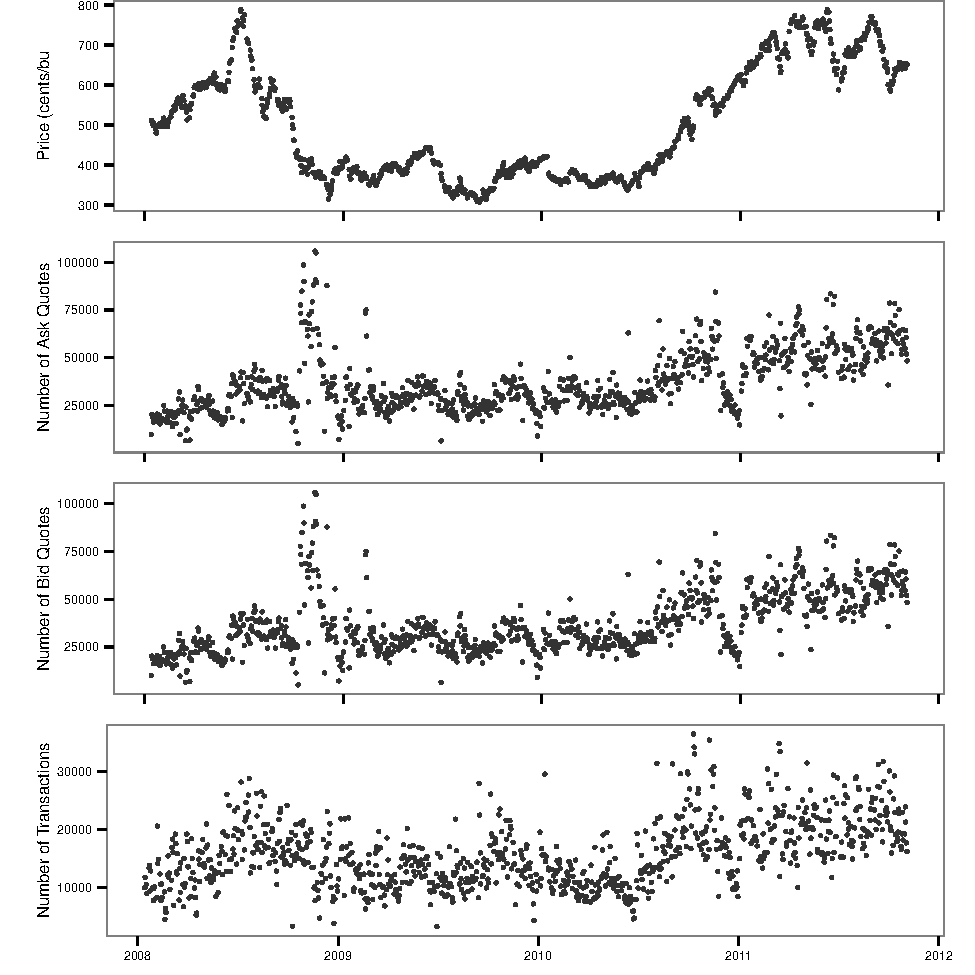
\includegraphics[scale=0.85]{TablesFigures_files/figure-latex/unnamed-chunk-3-1.pdf}
{\footnotesize \emph{Notes:} Figure displays data for the corn futures market from 1/14/2008 to
11/04/2011 for the nearby contract. The September contract is excluded
due to the possibility of `old crop' and `new crop' both being delivered
on this contract. To form the continuous nearby series contracts are
rolled to the next contract on the 20th of the month prior to the
delivery month. \par}
\caption{Price Levels, Number of Ask Quotes, Number of Bid Quotes, and
Number of Transactions}

\end{figure}


\clearpage

\begin{figure}[htbp]
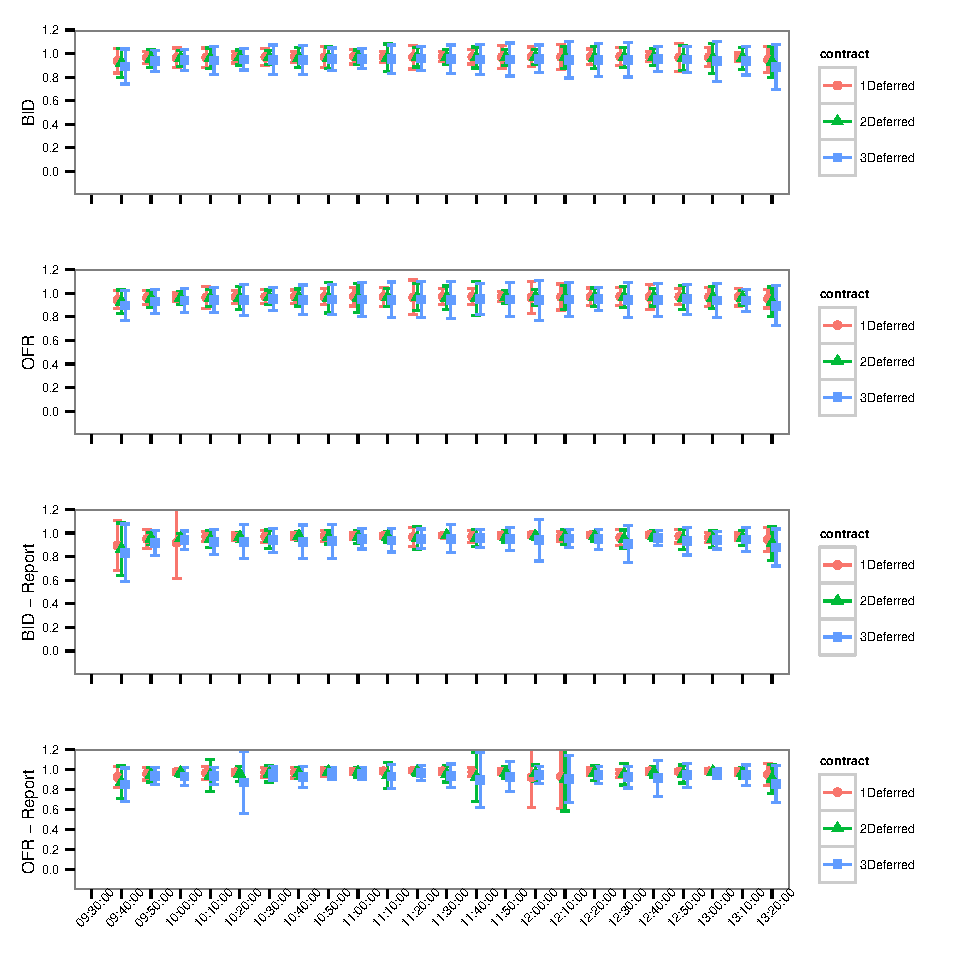
\includegraphics[scale=0.95]{TablesFigures_files/figure-latex/unnamed-chunk-4-1.pdf}
{\footnotesize  \emph{Notes:} Mean correlations and one standard deviation error bars over all days
are shown in the top two plots; report days only are included in the
bottom two plots. \par}
\caption{Information-Based Trading Activity and Contemporaneous
Correlations in the Top of the Book}
\end{figure}


\clearpage

\begin{figure}[htbp]
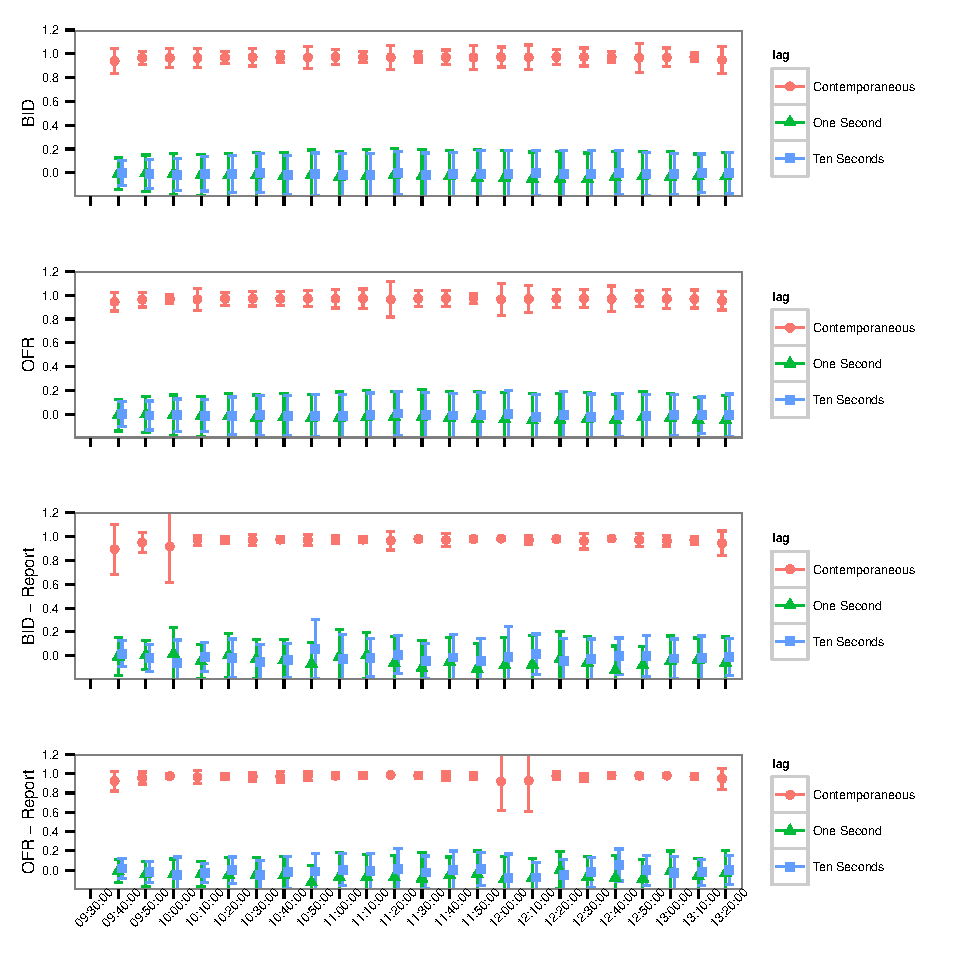
\includegraphics[scale=0.95]{TablesFigures_files/figure-latex/unnamed-chunk-5-1.pdf}
{\footnotesize  \emph{Notes:} Mean correlations and one standard deviation error bars over all days
are shown in the top two plots; report days only are included in the
bottom two plots. \par}
\caption{Speed of Information Transmission and Time-Lagged Correlations
in the Top of the Book}
\end{figure}


\clearpage

\begin{figure}[htbp]
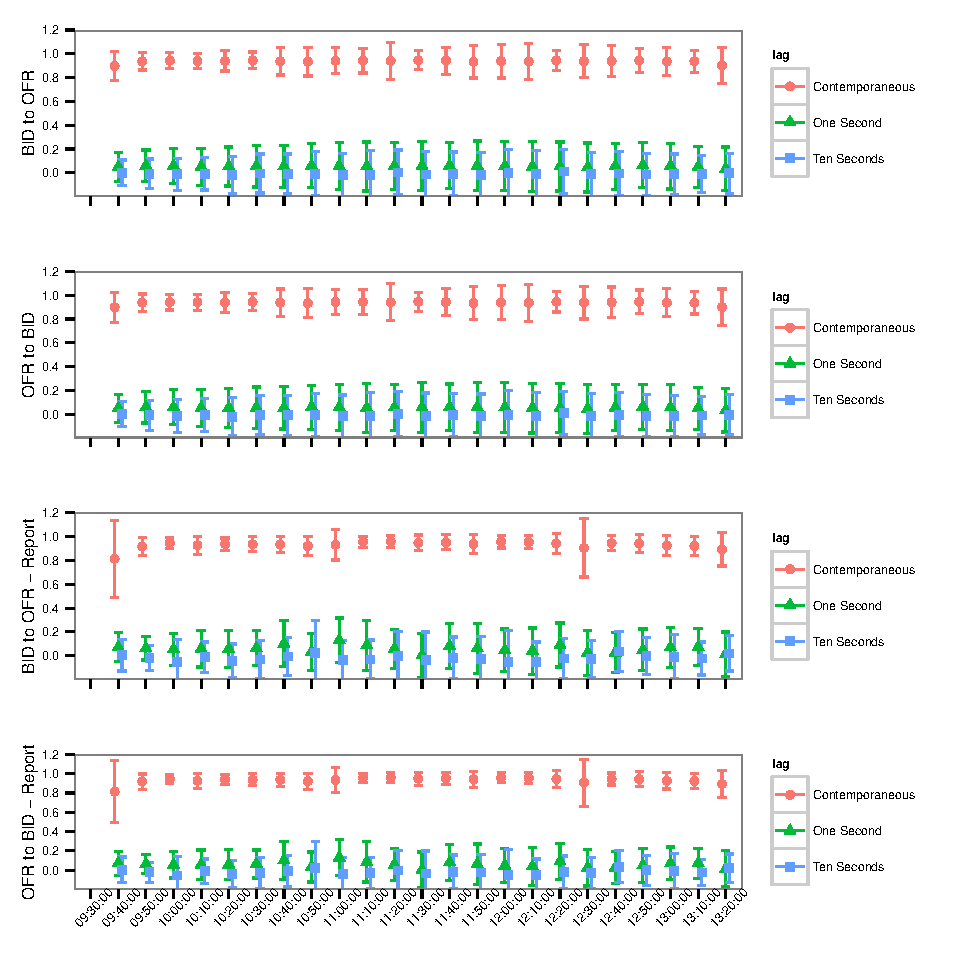
\includegraphics[scale=0.95]{TablesFigures_files/figure-latex/unnamed-chunk-6-1.pdf}
{\footnotesize  \emph{Notes:} Mean correlations and one standard deviation error bars over all days
are shown in the top two plots; report days only are included in the
bottom two plots. Bid-to-Offer shows correlation between revisions to
the lagged nearby bid and the first deferred revisions to the offer, and
Offer-to-Bid shows correlation between revisions to the lagged nearby
offer and the first deferred revisions to the bid. \par}
\caption{Spread Trades, Information Transmission, and Time-Lagged
Bid-to-Offer (Offer-to-Bid) Correlations}
\end{figure}






\end{document}